\section{\ExercisePrefixEmbeddedC Touchscreen ansteuern \optional}
Eingebaut im mit dem Microcontroller verbundenen Bildschirm ist eine resistive 4-Wire Touchschicht.
Der Name setzt sich zusammen aus den Eigenschaften dieser Schaltung.
Resistiv steht für die Messung von Widerständen zum Erkennen von Touch-Gesten und 4-Wire bedeutet, dass für diese Technik vier Datenleitungen gebraucht werden.
Ein resistiver 4-Wire-Touchscreen ist wie in Abbildung \ref{fig:rsTouch} aufgebaut.

\begin{figure}[!htb]
    \centering
    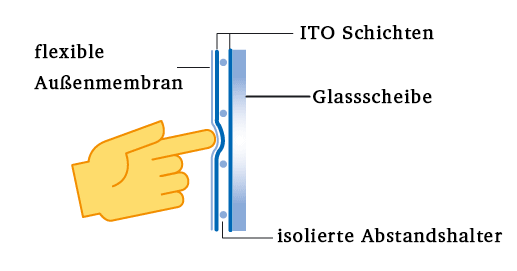
\includegraphics[width=0.35\textwidth]{./05_c/figures/4WireRSTouch.png}
    \caption{Aufbau eines resistiven Touchscreens}
    \label{fig:rsTouch}
\end{figure}

Dieser besteht aus
\begin{inparaenum}
\item
einer Glas- oder Acryl-Schicht,
\item 
einer äußeren resistiven Schicht, die mit Indium-Zinn-Oxid (\enquote{indium tin oxide}, ITO) beschichtet ist,
\item 
isolierenden Punkten,
\item 
der inneren resistiven Schicht aus ITO und 
\item
einem Polyester-Film.
\end{inparaenum}
Die beiden resistiven Schichten sind jeweils an 2 Polen angeschlossen (Abbildung \ref{fig:fourRSTouch}).

\begin{figure}[!htb]
    \centering
    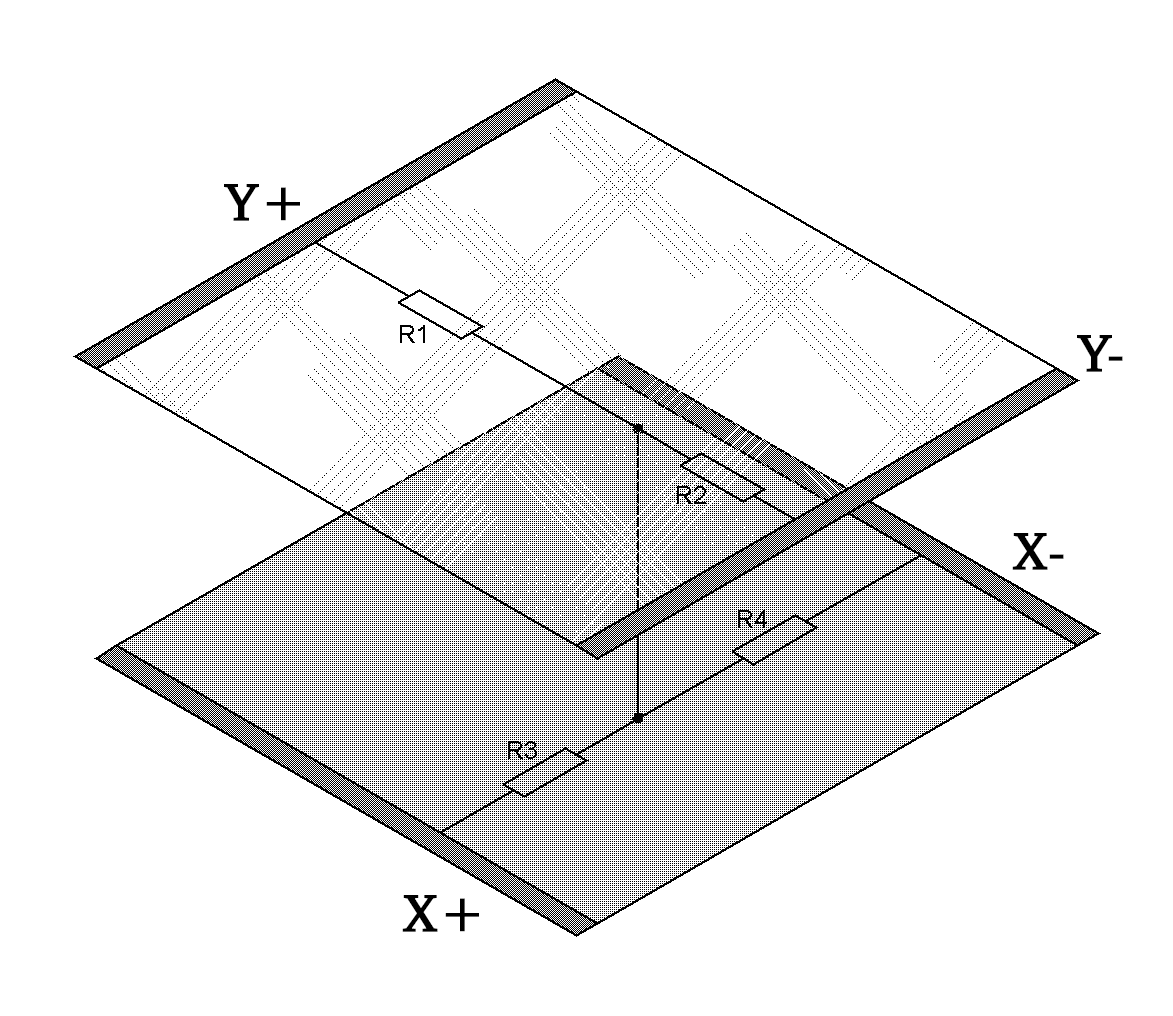
\includegraphics[width=0.3\textwidth]{./05_c/figures/ResistiveTS.png}
    \caption{Aufbau eines 4-Wire resistiven Touchscreens }
    \label{fig:fourRSTouch}
\end{figure} 

Die Schichten sind in Bezug auf ihre Pole um 90 Grad zueinander gedreht.
Dies ist wichtig, um später die X- und Y-Koordinaten des Druckpunkts zu lesen.
Sobald ein Objekt die oberste Glas- oder Acryl-Schicht berührt und genügend Druck ausübt, wird sich die oberste ITO-Schicht mit der unteren verbinden.
Die X- und Y-Koordinate des Druckpunkts wird bestimmt, indem die Spannungen an den Polen gemessen werden.
Zur Messung des X-Wertes werden X+ und X- über Gleichspannung geschaltet.
Das heißt, X+ ist beispielsweise auf Vcc und X- ist mit GND verbunden.
Durch die Verbindung der beiden ITO-Schichten entsteht ein Stromfluss durch beide Schichten und es kommt zu einem Spannungsteiler in der X-Schicht.
Die Spannungen zwischen X+ und dem Druckpunkt sowie dem Druckpunkt und X- lassen sich durch das Ausmessen von Y- und Y+ bestimmen.
Diese Information wird vom Microcontroller ausgelesen, der die gemessene Spannung in Relation zur Auflösung des Displays setzt.
Die Y-Koordinate wird gemessen, indem Y+ und Y- an eine Gleichspannung gelegt und die Spannungen an X+ und X- ausgelesen werden.

Für dein Projekt stellen wir dir die Funktionen \lstinline|cppp_readTouchX()|, \lstinline|cppp_readTouchY()| und \lstinline|cppp_readTouchZ()| zur Verfügung, die X-, Y- und Z-Werte eines Druckpunkts auf dem Touchscreen auslesen können (\filename{analog.h}).
Ist der Z-Wert größer als ein bestimmter Grenzwert, kann von einer Berührung des Touchscreens ausgegangen werden. 


\subsection{Werte des Touchscreens debuggen}
Implementiere zunächst die Funktion \lstinline|debugTouch()|, die kontinuierlich die X-,Y- und Z-Werte des Touchscreens auf dem Bildschirm ausgibt.

\subsection{Zeichnen auf dem Touchscreen}
In diesem Abschnitt implementierst du eine kleine Mal-Anwendung für den Touchscreen.
Mit dieser soll es möglich sein, verschiedene Farben auszuwählen und mithilfe des Fingers auf dem Bildschirm zu zeichnen.
Vervollständige hierfür die Funktion \lstinline|paintTouch()| sowie \lstinline|loopPaintTouch()|.
Bereits implementiert sind die Farbpaletten und der Lösch-Button auf der unteren Seite des Bildschirms.
Die Funktion \lstinline|loopPaintTouch()| muss noch um eine Touch-Logik ergänzt werden, die Berührungspunkte auf dem Bildschirm erkennt und diese korrekt interpretiert.
Hierbei gibt es folgende Szenarien:
\begin{itemize}
\item 
Die Farbpalette wird berührt und somit verändert sich die aktuelle Malfarbe.
\item 
Bild erneuern wurde gedrückt und der Malbereich wird zurückgesetzt.
\item 
Wird der freie Zeichen-Bereich berührt, so soll an dieser Stelle in der ausgewählten Farbe ein ausgefüllter Kreis mit dem Radius \lstinline|PENRADIUS| gezeichnet werden.
\end{itemize}
Abbildung \ref{fig:paintTouch} zeigt, wie die fertige Anwendung aussehen kann.
\begin{figure}[!htb]
	\centering
	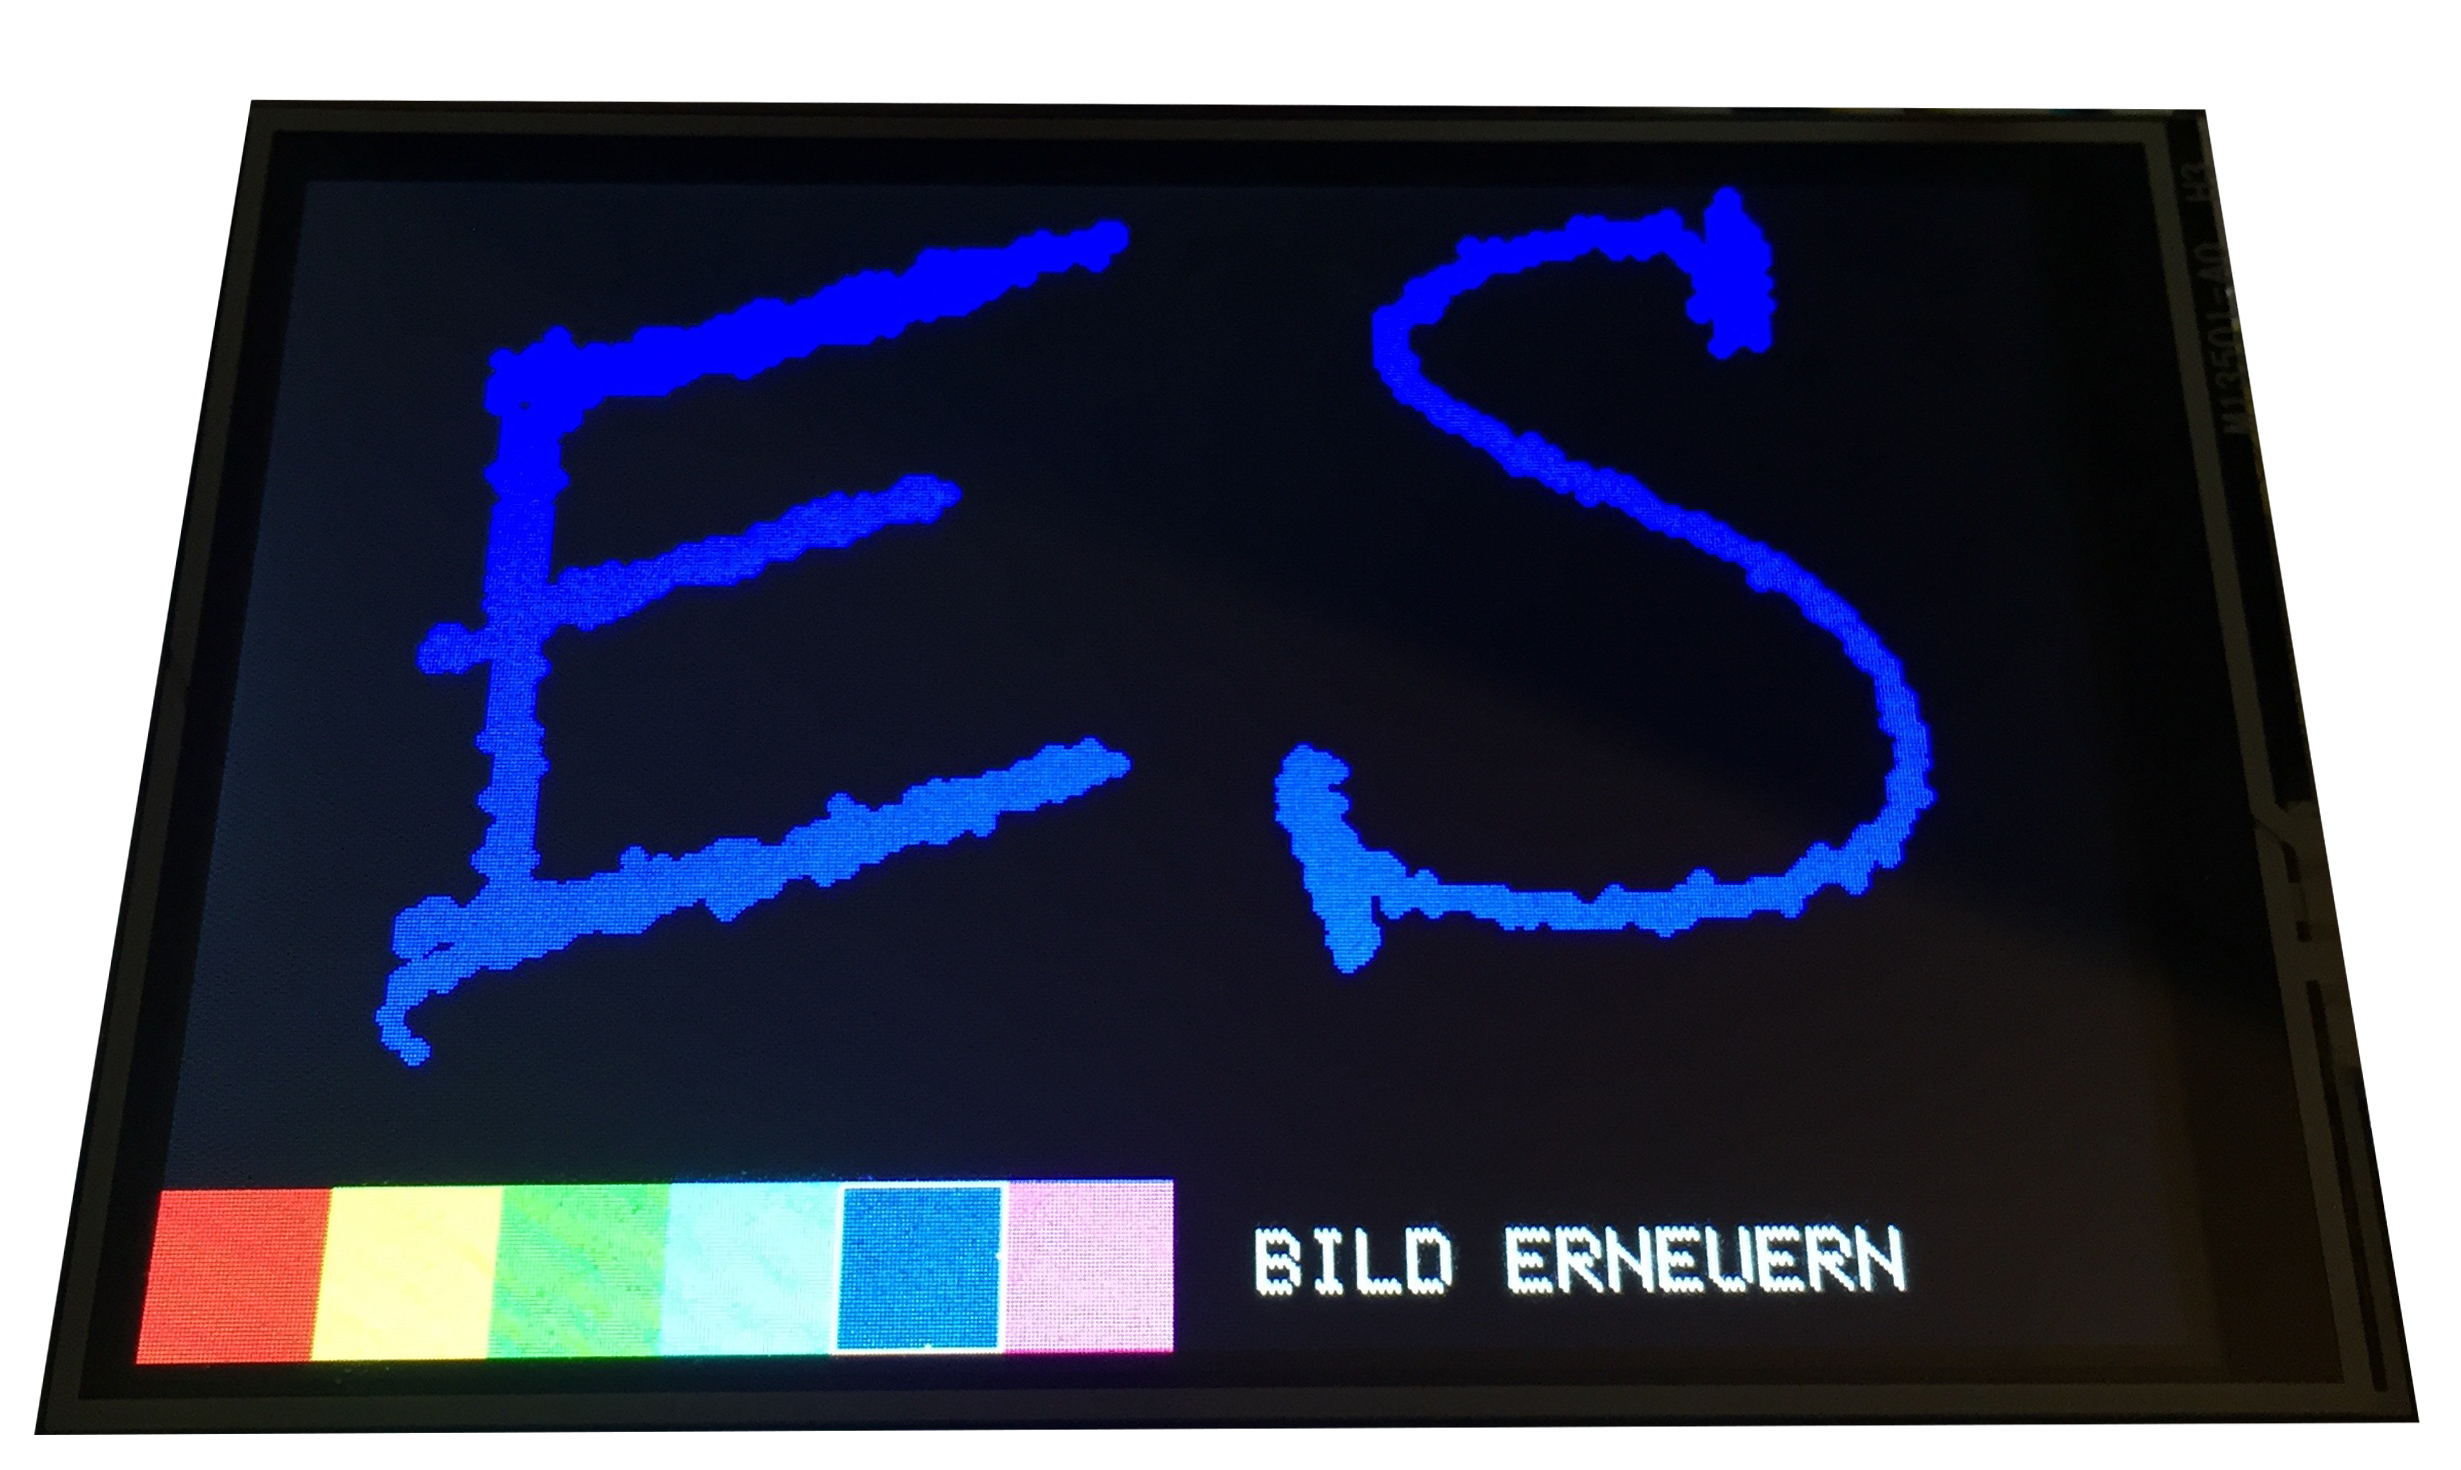
\includegraphics[width=0.3\textwidth]{./05_c/figures/Paint-Szenario.png}
	\caption{Mal-Anwendung auf dem Touchscreen}
	\label{fig:paintTouch}
\end{figure} 